\documentclass[10pt, a5paper]{article}
\usepackage{pdfpages}
\usepackage{parallel}
\usepackage[T2A]{fontenc}
\usepackage{ucs}
\usepackage[utf8x]{inputenc}
\usepackage[polish,english,russian]{babel}
\usepackage{hyperref}
\usepackage{rotating}
\usepackage[inner=2cm,top=1.8cm,outer=2cm,bottom=2.3cm,nohead]{geometry}
\usepackage{listings}
\usepackage{graphicx}
\usepackage{wrapfig}
\usepackage{longtable}
\usepackage{indentfirst}
\usepackage{array}
\newcolumntype{P}[1]{>{\raggedright\arraybackslash}p{#1}}
\frenchspacing
\usepackage{fixltx2e} %text sub- and superscripts
\usepackage{icomma} % коскі ў матэматычным рэжыме
\PreloadUnicodePage{4}

\newcommand{\longpage}{\enlargethispage{\baselineskip}}
\newcommand{\shortpage}{\enlargethispage{-\baselineskip}}

\def\switchlang#1{\expandafter\csname switchlang#1\endcsname}
\def\switchlangbe{
\let\saverefname=\refname%
\def\refname{Літаратура}%
\def\figurename{Іл.}%
}
\def\switchlangen{
\let\saverefname=\refname%
\def\refname{References}%
\def\figurename{Fig.}%
}
\def\switchlangru{
\let\saverefname=\refname%
\let\savefigurename=\figurename%
\def\refname{Литература}%
\def\figurename{Рис.}%
}

\hyphenation{admi-ni-stra-tive}
\hyphenation{ex-pe-ri-ence}
\hyphenation{fle-xi-bi-li-ty}
\hyphenation{Py-thon}
\hyphenation{ma-the-ma-ti-cal}
\hyphenation{re-ported}
\hyphenation{imp-le-menta-tions}
\hyphenation{pro-vides}
\hyphenation{en-gi-neering}
\hyphenation{com-pa-ti-bi-li-ty}
\hyphenation{im-pos-sible}
\hyphenation{desk-top}
\hyphenation{elec-tro-nic}
\hyphenation{com-pa-ny}
\hyphenation{de-ve-lop-ment}
\hyphenation{de-ve-loping}
\hyphenation{de-ve-lop}
\hyphenation{da-ta-ba-se}
\hyphenation{plat-forms}
\hyphenation{or-ga-ni-za-tion}
\hyphenation{pro-gramming}
\hyphenation{in-stru-ments}
\hyphenation{Li-nux}
\hyphenation{sour-ce}
\hyphenation{en-vi-ron-ment}
\hyphenation{Te-le-pathy}
\hyphenation{Li-nux-ov-ka}
\hyphenation{Open-BSD}
\hyphenation{Free-BSD}
\hyphenation{men-ti-on-ed}
\hyphenation{app-li-ca-tion}

\def\progref!#1!{\texttt{#1}}
\renewcommand{\arraystretch}{2} %Іначай формулы ў матрыцы зліпаюцца з лініямі
\usepackage{array}

\def\interview #1 (#2), #3, #4, #5\par{

\section[#1, #3, #4]{#1 -- #3, #4}
\def\qname{LVEE}
\def\aname{#1}
\def\q ##1\par{{\noindent \bf \qname: ##1 }\par}
\def\a{{\noindent \bf \aname: } \def\qname{L}\def\aname{#2}}
}

\def\interview* #1 (#2), #3, #4, #5\par{

\section*{#1\\{\small\rm #3, #4. #5}}

\def\qname{LVEE}
\def\aname{#1}
\def\q ##1\par{{\noindent \bf \qname: ##1 }\par}
\def\a{{\noindent \bf \aname: } \def\qname{L}\def\aname{#2}}
}

\begin{document}
\title{Голос спонсора: Promwad}
%\author{}
\date{}
\maketitle
%\begin{wrapfigure}{l}{0.3\textwidth}

\begin{figure}[h!]
\centering
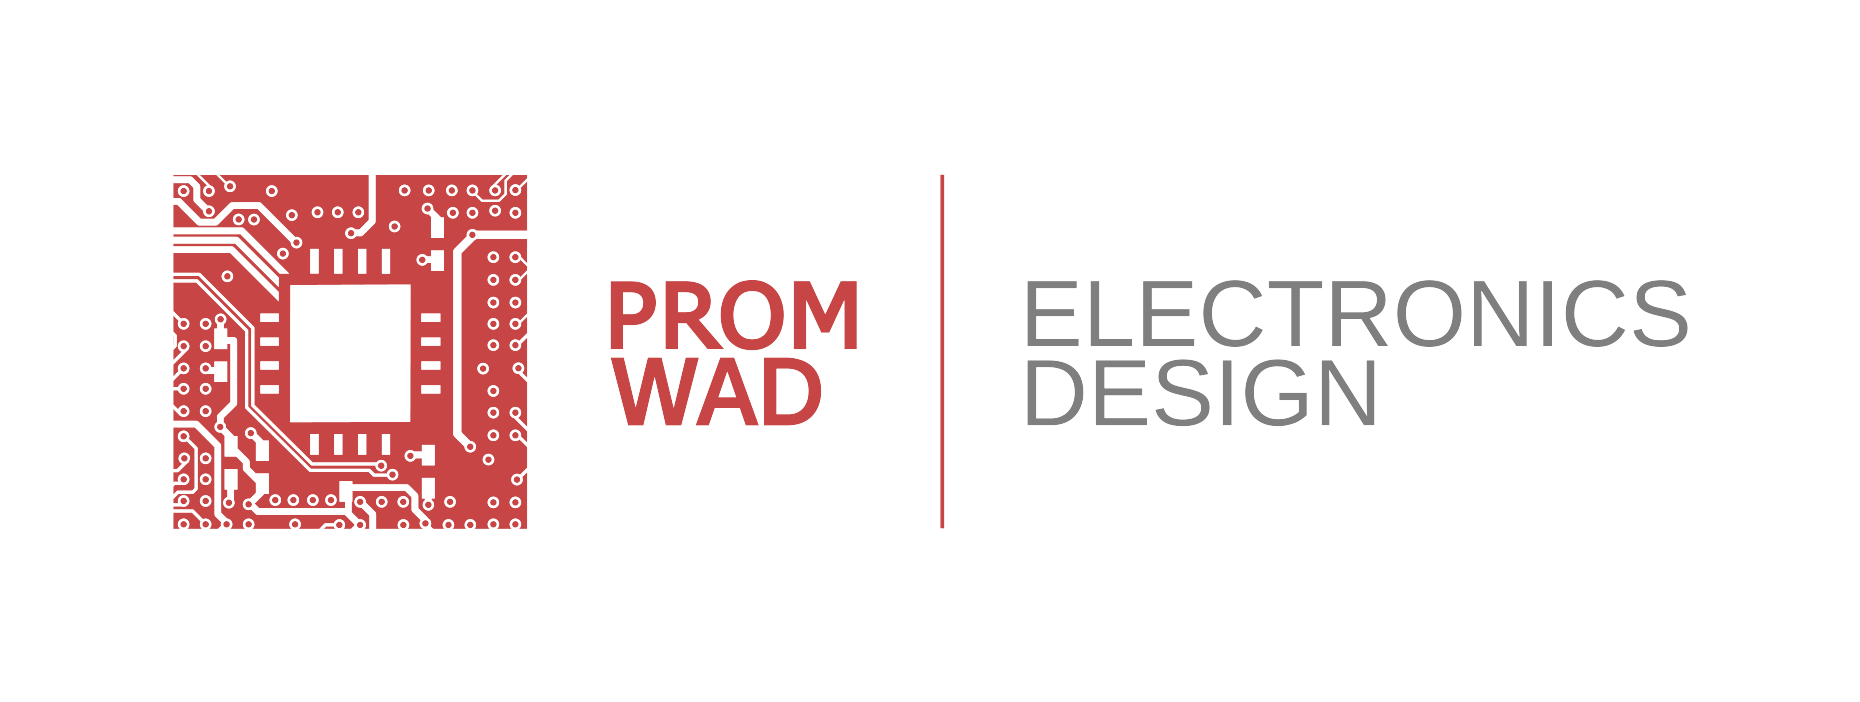
\includegraphics[width=10cm]{53_spons_promwad.png}
\end{figure}

{\bf Инновационная компания Promwad} реализует полный цикл разработки электроники: создание концепции продукта, промышленный дизайн и конструирование, проектирование аппаратных \linebreak платформ, разработка встроенного и прикладного ПО, тестирование ПО и контроль качества, сертификация, изготовление опытных образцов, постановка и сопровождение массового производства.

Promwad предлагает услуги аутсорсинга разработки электронных устройств в различных отраслях рынка электроники: телекоммуникации, автомобильная электроника, автоматизация, потребительская электроника, медиа и развлечения и другие. 

Разработка встроенного ПО "--- одна из основных услуг и направлений развития Promwad. Мы разрабатываем ПО для микропроцессоров, систем-на-кристалле, цифровых сигнальных процессоров и микроконтроллеров.

Наши разработчики работают с:
\begin{itemize}
\item Операционными системами "--- GNU/Linux, Android, FreeRTOS, RTEMS и другие специализированные RTOS
\item Языками программирования "--- C (user-space, kernel-space),\linebreak ARM Assembler, C++, Unix shell, Lua, Python, Javascript
\item Графическими библиотеками "--- QT+QML, SDL, OpenGL
\item Linux подсистемами "--- network drivers, USB, PCI, UART, SPI, I2C, GPIO, IRQs, Real time scheduling, cryptography, DMA, PMIC, ALSA, touchscreen, sensors, framebuffer, v4l2
\item Базами данных "--- MySQL, sqlite
\item Средствами сборки "--- make, Automake/Autotools, Cmake, \linebreak Qmak
\item Сборочными системами, фреймворками "--- Buildroot, \linebreak OpenEmbedded, Yocto, Openwrt, rpm/rpmbuild, deb/debuild, uClinux, STAPI
\item Отладками "--- jtag, openocd, valgrind, gdb
\item Системами контроля версий "--- SVN, GIT
\end{itemize}

В компании всегда открыт набор специалистов- разработчиков Linux Embedded, имеющих опыт работы  на языке программирования С/С++  в сфере Embedded не менее двух лет.

Сегодня Promwad "--- это успешная компания на рынке электроники и IT, резидент Парка высоких технологий (ПВТ), участник партнерских программ ведущих мировых производителей электронных компонентов, таких как Texas Instruments, STMicroelectronics, Analog Devices, Marvell и Fujitsu. 

Как современная компания мы уделяем внимание внутренним ценностям: обучение, развитие сотрудников, активный отдых, спонсорство и участие в тематических конференциях и тп. (с 2007 года Promwad постоянный спонсор конференций LVEE, а с 2009 года проводит собственный Форум разработчиков цифровой электроники "--- DEDF).

Как социально ответственная компания мы являемся партнером и титульным спонсором Кубка приключенческих гонок "--- ПромвадТур, который объединяет неравнодушных к активному досугу и приключениям единомышленников различных профессий. 

Описание услуг  компании, портфолио выполненных проектов, текущие вакансии и другую полезную информацию смотрите на корпоративном сайте Promwad: \url{www.promwad.com}.

{\bf Мы любим то, что делаем, и работаем на результат! Если ты разделяешь нашу позицию "--- будем рады принять в команду!}
